\documentclass{article}

\usepackage[a4paper,textwidth=16cm]{geometry}
\usepackage{mathtools}
\usepackage{graphicx,fancyhdr}
\usepackage{enumitem}

\pagestyle{fancy}

\fancypagestyle{plain}{ %
  \fancyhf{} % remove everything
  \renewcommand{\headrulewidth}{0pt} % remove lines as well
  \renewcommand{\footrulewidth}{0pt}
}

\lhead{02616 -- Large Scale Modelling}
\chead{}
\rhead{Fall}
\lfoot{}
\rfoot{}

\setitemize{itemsep=-3pt}

\newcommand\code[1]{\texttt{#1}}

\begin{document}
\begin{center}
\fbox{Your report (PDF) and the required sources (ZIP)  must be handed in electronically!}
\fbox{Deadline: latest on Sunday, October 18, 2026 at midnight!}
\end{center}

\section*{Project 1 -- Mandelbrot}

In our first project of Large Scale Modelling
we will implement the Mandelbrot set calculation.

The Mandelbrot set can be calculated for a given
pixel using a truncation function:
\begin{align}
  p_0 &= x + iy
  \\
  p_{n+1} &= p_n^2 + p_0
\end{align}
where $x$ and $y$ are the image coordinates, and $i$ is the imaginary number.
The iteration is truncated when $|p_{n}| > 2$ or $n> n_{\mathrm{max}}$.
Then store $n$ (or use some color palette of the number of iterations) in the image.

The outer-most Mandelbrot set is defined in the image limits:
\begin{align}
x &\in [-2.2, 0.75]
\\
y &\in [-1.3, 1.3].
\end{align}

\begin{figure}[!h]
  \centering
  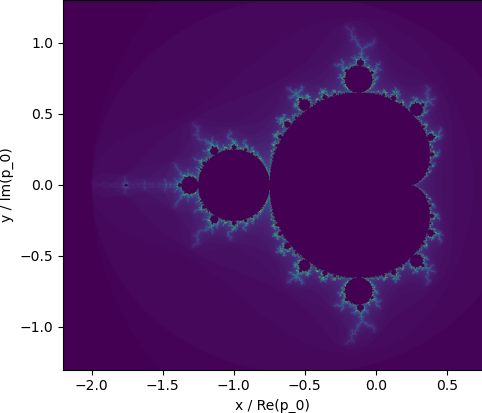
\includegraphics[width=0.7\textwidth]{Figure_1}
  \caption{An image of the Mandelbrot set in the default view-range.}
\end{figure}


Please extend the shipped \code{Mandelbrot.py} code to use
MPI and if additional arguments are necessary, add them to the end
of the argument list.

With the current flags you can investigate several different
regions of the image and thus scour its inherent load imbalance
problems.


\subsection*{Expected investigations}

The Mandelbrot example is a case of a compute-bound problem
with load-imbalance.
We expect you to at least have 2 different MPI implementations:
\begin{itemize}
  \item a blocking send/receive code
  \item a non-blocking send/receive code
\end{itemize}

In both cases they should be implemented using a row-only
distribution, i.e. the image is updated along the rows (x coordinate) of the array.
You may later investigate/describe other work distributions.
Use the \texttt{chunk-size} variable in the shipped code to
create an initial load-distribution algorithm.
We expect that you present a report with at least the following
surveys:

\begin{itemize}
  \item Discuss, implement and analyse different load balancing strategies.

    For instance, one could implement a static scheduler (each rank gets
    a pre-determined chunk-segment), or one could implement a dynamic
    scheduler (where work is \emph{requested} by the workers).

    There is a lot of freedom in choosing
    how to distribute work, \emph{remember} to describe
    the distribution in common language.

    \begin{quote}
      We prefer deep analysis of a few distributions vs.
      a weak analysis on many distributions!
      This is not a programming competition!
    \end{quote}

    If there is not enough time for implementing a dynamic scheduling,
    discuss how one could imagine it being implemented.


  \item A performance benchmark of the different implementations.
    E.g. scalability plots, possibly with different load balancing
    strategies.

    \begin{quote}
      Explain why you get the plots you get!
    \end{quote}

  \item A performance benchmark when using 1 node vs. multiple nodes. Hint:
    the size of the image, i.e. the number of pixels, has an influence on
    different performance aspects here!

  \item Discuss code-progress and changes in the code by showing small code-snippets
    in the report, and how the changes influence the performance (either worsen or
    improves).

\end{itemize}


\subsection*{Notes}
\begin{itemize}
  \item Labels on figures, and explanatory figure captions!
  \item Ensure your lines on graphs are distinguishable.
  \item Consider what you are timing, and what you compare.
  \item Please write the report so your fellow students (not taking the
    course) can understand it.
  \item Ensure to explain why you see things, if a scalability plot
    that flattens has a reason, what's the reason?
    Saying ``The method scales up to 4 cores.'' is not a reason! :)
  \item Make a plan of the things you want to investigate,
    it's easy to throw a lot of jobs at the cluster. Instead, estimate
    how long time all the jobs will take.
    Say, if you want to test for $N$ core configurations, $P$ parameters
    and each run takes 4 min on average, that amounts to $4 N P$
    minutes. You only have a limited amount of time to conduct experiments,
    \emph{AND} you also have to write the report. Planning is key here!
  \item Labels on figures, and explanatory figure captions! (purposefully duplicated!)

  \item Use AI responsibly! Making mistakes is a \emph{good} thing. Let us see what
    \emph{you} can write!

\end{itemize}

\subsection*{Upload}
\begin{itemize}
  \item your report in PDF format
  \item a ZIP files with the Python sources, that are needed to run your code, remember to
    tell us how to execute it.
\end{itemize}

\end{document}
